\documentclass[conference]{IEEEtran}
\IEEEoverridecommandlockouts
% The preceding line is only needed to identify funding in the first footnote. If that is unneeded, please comment it out.
\usepackage{cite}
\usepackage{amsmath,amssymb,amsfonts}
\usepackage{algorithmic}
\usepackage{graphicx}
\usepackage{textcomp}
\usepackage{xcolor}
\usepackage{tabularx}
\usepackage{hyperref}
\usepackage{url}
\usepackage{xurl}
\def\BibTeX{{\rm B\kern-.05em{\sc i\kern-.025em b}\kern-.08em
    T\kern-.1667em\lower.7ex\hbox{E}\kern-.125emX}}
\begin{document}

\title{Trustless by Design: A New Architecture for Peer-to-Peer Accommodation Platform}

\author{\IEEEauthorblockN{Ceavin Rufus De Prayer Purba}
\IEEEauthorblockA{\textit{School of Electrical Engineering and Informatics} \\
\textit{Institut Teknologi Bandung}\\
Bandung, Indonesia \\
ceavinr@gmail.com}
}

\maketitle

\begin{abstract}
The growing demand for online accommodation systems highlights critical vulnerabilities in conventional centralized transaction models, which often compromise user privacy and foster inefficient third-party dependencies. This research proposes a novel, fully anonymous, and decentralized peer-to-peer accommodation platform designed with a "trustless" architecture, where user identity is paramount. Employing a Design Science Research Methodology (DSRM), the system integrates smart contracts for automated, transparent transactions, and leverages Self-Sovereign Identity (SSI) with Zero-Knowledge Proof (ZKProof) to ensure robust privacy protection. All transaction phases, from booking to dispute resolution, are executed via smart contracts, eliminating third-party intermediaries. SSI and ZKProof enable users to prove access rights through anonymous booking credentials without disclosing personal data, while decentralized cryptographic proofs ensure anonymous user uniqueness and validity. As a proof of concept, the implemented system demonstrates transparent, secure, and fully anonymous accommodation booking.
\end{abstract}

\begin{IEEEkeywords}
design science research, peer-to-peer, blockchain, smart contract, zero-knowledge proof, verifiable credential, self-sovereign identity, privacy-preserving identity
\end{IEEEkeywords}

\section{Introduction}
\label{sec:introduction}
The global tourism industry has experienced significant growth in recent years, with peer-to-peer accommodation platforms (P2P APs) such as Airbnb transforming how travelers find lodging. In Indonesia alone, 1.34 million international and over 75 million domestic tourists were recorded as of August 2024 (Badan Pusat Statistik). However, most existing P2P APs rely on centralized architectures, where sensitive user data such as identity, payment, and behavior history is stored and controlled by a single service provider \cite{rosoon2023, raj2019}. This centralization creates various risks, including data breaches \cite{rundle2024, malcolm2024}, censorship and moderation bias \cite{blengini2024}, and unbalanced control over reputation and access systems \cite{hawlitschek2018}.

Security and privacy concerns in centralized platforms significantly affect user trust, which is essential in P2P systems where transactions occur between strangers \cite{mayer1995, oliveira2017, agag2019}. Although existing platforms incorporate reputation mechanisms such as user reviews and ratings to build trust, these systems often suffer from manipulation, bias, and cold-start limitations \cite{tussyadiah2018, zloteanu2021, huang2021}. Additionally, reliance on third-party intermediaries like payment processors increases operational overhead and introduces additional vulnerabilities \cite{hawlitschek2018, bhushan2021}.

Decentralized technologies offer promising alternatives to address these challenges. Blockchain enables transparent, tamper-resistant interactions without relying on central authorities \cite{nakamoto2008, wood2022}. Smart contracts facilitate self-executing agreements on the blockchain without the need for intermediaries \cite{buterin2014, bhushan2021}. Self-sovereign identity (SSI) gives users full control over their personal data and credentials, allowing them to selectively disclose information \cite{wang2019, raipurkar2023, mittal2025}. Zero-knowledge proofs (ZKPs) further enhance user privacy by enabling proof of claims without exposing any underlying data \cite{dieye2023, chen2022, moya2023}.

This paper presents the design and implementation of a trustless, privacy-preserving P2P accommodation platform that integrates smart contracts, SSI, and ZKPs. The system allows users to make anonymous bookings and verify access rights without requiring the platform to store identity information. Using verifiable credentials and ZKPs, users can cryptographically prove they are unique, verified, and eligible to book, while maintaining anonymity \cite{lux2020, sporny2022, reed2020}.

This research adopts the Design Science Research Methodology (DSRM) \cite{peffers2007, venable2017} to guide the development process. The problem is analyzed from four dimensions: privacy vulnerabilities in centralized storage, reliance on third parties for trust and payments, the trade-off between transparency and privacy, and the shortcomings of conventional reputation systems. The solution presented aims to demonstrate that it is feasible to build a more secure, transparent, and user-centric P2P accommodation platform based on decentralized identity and cryptographic trust.

\section{State of the Art}
\label{sec:state-of-the-art}
This section presents a literature review and theoretical foundation that supports the development of a decentralized peer-to-peer accommodation platform. It explores the concepts of peer-to-peer platforms, digital identity, blockchain technologies, trust frameworks, and cryptographic privacy-preserving methods, particularly zero-knowledge proofs and self-sovereign identity (SSI).

\subsection{Peer-to-Peer Accommodation Platforms}
Peer-to-peer accommodation platforms (P2P AP) are part of the broader sharing economy that enables individuals to rent out their available spaces through online platforms \cite{cesnuityte2022}. These platforms operate under both commercial models (e.g., Airbnb) and non-commercial models (e.g., Couchsurfing). While commercial models prioritize transaction efficiency and monetization, both models face challenges related to user privacy, data security, and trust between transacting parties.

\subsection{Digital Identity}
Digital identity represents a collection of attributes, identifiers, and credentials used to establish a user’s presence in online environments \cite{wang2019}. Traditional identity systems rely on centralized providers, which introduces vulnerabilities such as data breaches and loss of user control. Concepts like persona, attributes, and identifiers play critical roles in modeling identity contexts in digital systems.

\subsection{Blockchain}
Blockchain is a decentralized ledger that maintains data integrity through consensus mechanisms and cryptographic linking of blocks \cite{nakamoto2008}. Ethereum, a prominent blockchain platform, supports decentralized applications (dApps) and enables smart contracts—self-executing programs that enforce agreements when predefined conditions are met \cite{buterin2014, wood2022, antonopoulos2019, bhushan2021}. These contracts, typically written in languages such as Solidity \cite{solidity2024}, are immutable and transparent once deployed, reducing reliance on intermediaries and minimizing the risk of manipulation in digital interactions \cite{raj2019}. Together, blockchain and smart contracts form the foundation for trustless, automated systems that support the secure execution of platform logic in decentralized environments.

\subsection{Trustless Systems}
Trust is a multidimensional concept essential in peer-to-peer systems where parties often interact without prior relationships. Mayer et al. define trust as the willingness to be vulnerable to another party’s actions without direct control \cite{mayer1995}. Xu et al. further classify trust into interpersonal, institutional, and technological trust—each playing a role in user decision-making and system adoption in digital environments \cite{xu2014}. In decentralized contexts, trust shifts toward confidence in the platform's reliability, security, and design.

Trustless systems aim to eliminate reliance on interpersonal or institutional trust by embedding assurance mechanisms directly into the system’s architecture, particularly using blockchain and smart contracts \cite{gan2024}. However, studies such as Hawlitschek et al. highlight that full trustlessness is difficult to achieve due to residual algorithmic trust and sociotechnical dependencies \cite{hawlitschek2018}. The effectiveness of trustless systems depends on secure code, protocol correctness, and regulatory legitimacy.

\subsection{Zero-Knowledge Proofs (ZKPs)}
ZKPs allow one party to prove possession of information to another party without revealing the information itself \cite{dieye2023}. zk-SNARKs, a non-interactive form of ZKPs, are highly efficient and widely used in blockchain privacy applications due to their succinctness and cryptographic soundness \cite{chen2022, moya2023}. These techniques are foundational to enabling privacy-preserving verification in decentralized systems.

\subsection{Self-Sovereign Identity (SSI)}
Self-Sovereign Identity (SSI) empowers users with full control over their digital identities, allowing them to manage, store, and present credentials in a decentralized and privacy-preserving manner \cite{raipurkar2023}. Unlike traditional identity systems that depend on centralized authorities, SSI gives individuals ownership of their personal data, minimizing reliance on third parties.

At the core of the SSI model are two primary components:

\begin{itemize}
  \item \textbf{Decentralized Identifiers (DIDs):} Unique identifiers stored on a blockchain or other decentralized network, enabling users to prove control over their identity without needing a central registry \cite{reed2020}.
  \item \textbf{Verifiable Credentials (VCs):} Digitally signed claims issued by trusted entities (issuers) to holders, who can present them to verifiers as proof of specific attributes or qualifications \cite{sporny2022}.
\end{itemize}

Verifiable Credentials offer enhanced privacy and data minimization through features like:
\begin{itemize}
  \item \textbf{Selective disclosure:} Holders can reveal only the specific data required by a verifier, without disclosing the full credential.
  \item \textbf{Zero-Knowledge Proofs (ZKPs):} Holders can prove statements about their credentials without revealing the underlying data (e.g., proving they are over 18 without sharing their birthdate).
\end{itemize}

Figure~\ref{fig:vc-work} illustrates how Verifiable Credentials work within the SSI trust model, involving three roles: \textit{issuer}, \textit{holder}, and \textit{verifier}. The issuer provides a credential to the holder, who stores it in a secure identity wallet. When required, the holder generates a verifiable presentation for the verifier, who checks its authenticity using the issuer’s public key and DID document.

\begin{figure}[ht]
    \centering
    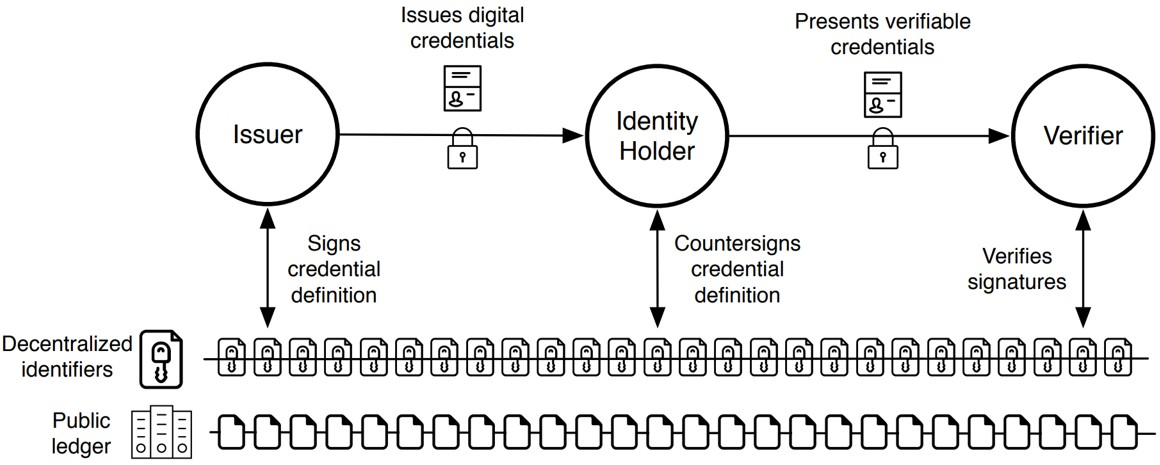
\includegraphics[width=0.99\linewidth]{how-vc-work.jpg}
    \caption{How verifiable credentials work in the SSI trust model \cite{lux2020}}
    \label{fig:vc-work}
\end{figure}

This approach eliminates the need for direct contact between verifier and issuer, supporting privacy-preserving, decentralized identity verification at scale. Verifiable Credentials are especially relevant in peer-to-peer platforms where users must prove claims (e.g., booking history, identity, or age) without compromising sensitive information.

\subsection{Trust Triangle}
The Self-Sovereign Identity (SSI) framework is structured around the “trust triangle,” comprising three roles: the \textbf{issuer}, the \textbf{holder}, and the \textbf{verifier}. In this model, issuers grant verifiable credentials (VCs) to holders, who store them securely and later present cryptographic proofs to verifiers. The trust triangle ensures decentralized yet trustworthy authentication without revealing sensitive user data \cite{sporny2022, lux2020}. 

Protocols like Iden3 and platforms such as Privado ID apply this model by combining zk-SNARK-based proof systems with decentralized identifier (DID) infrastructure \cite{iden3docs, mittal2025}. Figure~\ref{fig:trust-triangle} illustrates the generalized flow of trust and data exchange in SSI-based systems, as adopted in this platform.

\begin{figure}[h!]
  \centering
  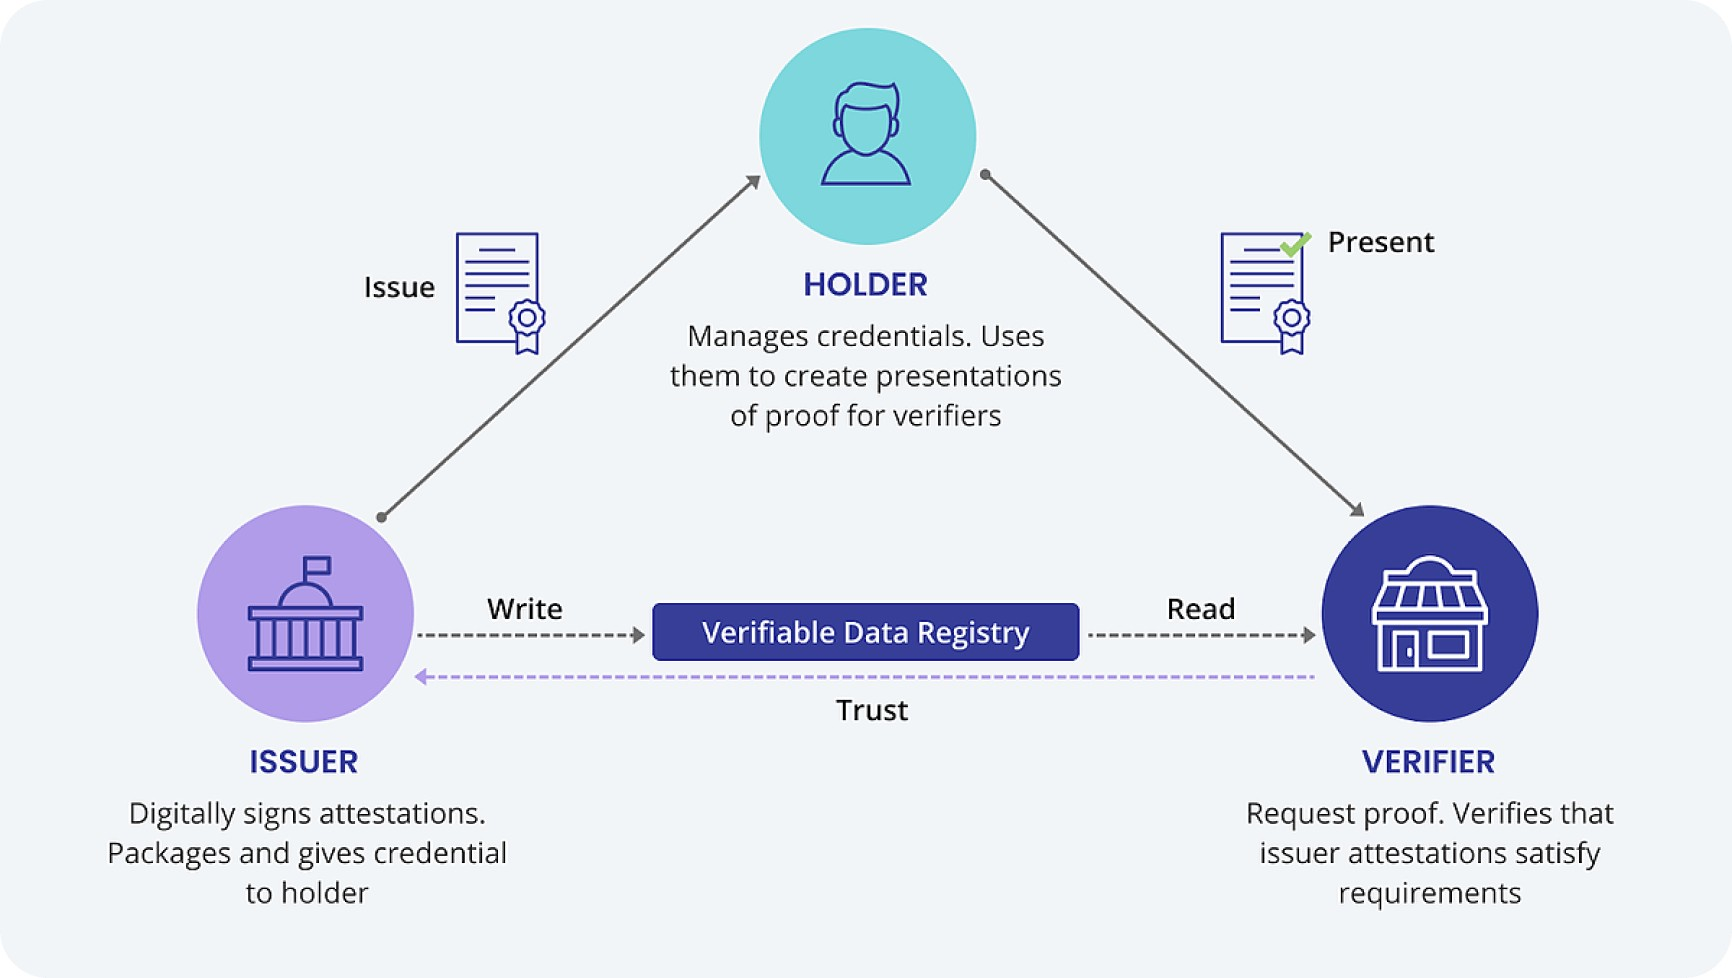
\includegraphics[width=1\linewidth]{trust-triangle.jpg}
  \caption{Illustration of the SSI trust triangle model showing the roles of Issuer, Holder, and Verifier. This diagram reflects the decentralized credential exchange and verification mechanism central to self-sovereign identity \cite{cheqd2023}.}
  \label{fig:trust-triangle}
\end{figure}

\section{Related Work}
\label{sec:related-work}
Trust is a critical component in peer-to-peer (P2P) accommodation platforms, where users must engage in transactions with unknown parties. Studies such as \cite{agag2019} and \cite{oliveira2017} emphasize the importance of institutional and interpersonal trust in user decision-making. However, traditional platforms rely heavily on centralized data management, which can introduce biases and manipulation in reputation systems \cite{hawlitschek2018, tussyadiah2018}. Attribution bias and misinformation can further degrade trust accuracy in online reviews \cite{huang2021, zloteanu2021}.

Blockchain has been explored as a trust infrastructure that removes the need for centralized intermediaries. Research by Hawlitschek et al. \cite{hawlitschek2018} and Dann et al. \cite{dann2020} suggest that distributed ledgers can replace institutional trust with technological trust. The Ethereum blockchain in particular has been used as a base for smart contract platforms, enabling secure and transparent automation of transactions \cite{buterin2014, wood2022, antonopoulos2019}.

Self-sovereign identity (SSI) has gained attention as a user-centric identity solution that removes reliance on third-party identity providers. SSI frameworks are based on decentralized identifiers (DIDs) and verifiable credentials (VCs), allowing users to present proof of identity or attributes without revealing sensitive data \cite{wang2019, reed2020, sporny2022}. SSI is especially relevant in the context of online platforms where users are concerned about surveillance and data misuse.

Zero-knowledge proofs (ZKPs) further enhance privacy by enabling users to prove possession of a credential or attribute without disclosing its content. ZKPs such as zk-SNARKs are being actively researched and applied in identity systems \cite{chen2022, dieye2023}. Several works propose the integration of ZKPs and SSI into blockchain-based access systems \cite{moya2023, raipurkar2023}, providing privacy-preserving mechanisms for authentication and access control.

While various approaches have explored blockchain and SSI individually, few implementations have combined these technologies specifically in the context of P2P accommodation. Our research fills this gap by proposing a holistic system that integrates smart contracts, verifiable credentials, and zero-knowledge proofs to enable privacy-preserving and decentralized booking on a trustless platform.

\section{System Design}
The proposed system is a decentralized peer-to-peer accommodation platform designed to address the trust, privacy, and transparency limitations of traditional platforms. It is built on top of blockchain smart contracts, integrates self-sovereign identity (SSI), and applies zero-knowledge proofs (ZKPs) to protect user privacy while ensuring eligibility and uniqueness.

\subsection{System Architecture Overview}
Figure~\ref{fig:architecture_diagram} illustrates the architecture of the system, showing how key components interact across three major layers: blockchain, SSI with ZKProof, and centralized infrastructure. This hybrid architecture balances decentralization, privacy, and practical scalability.

\begin{figure}[h!]
  \centering
  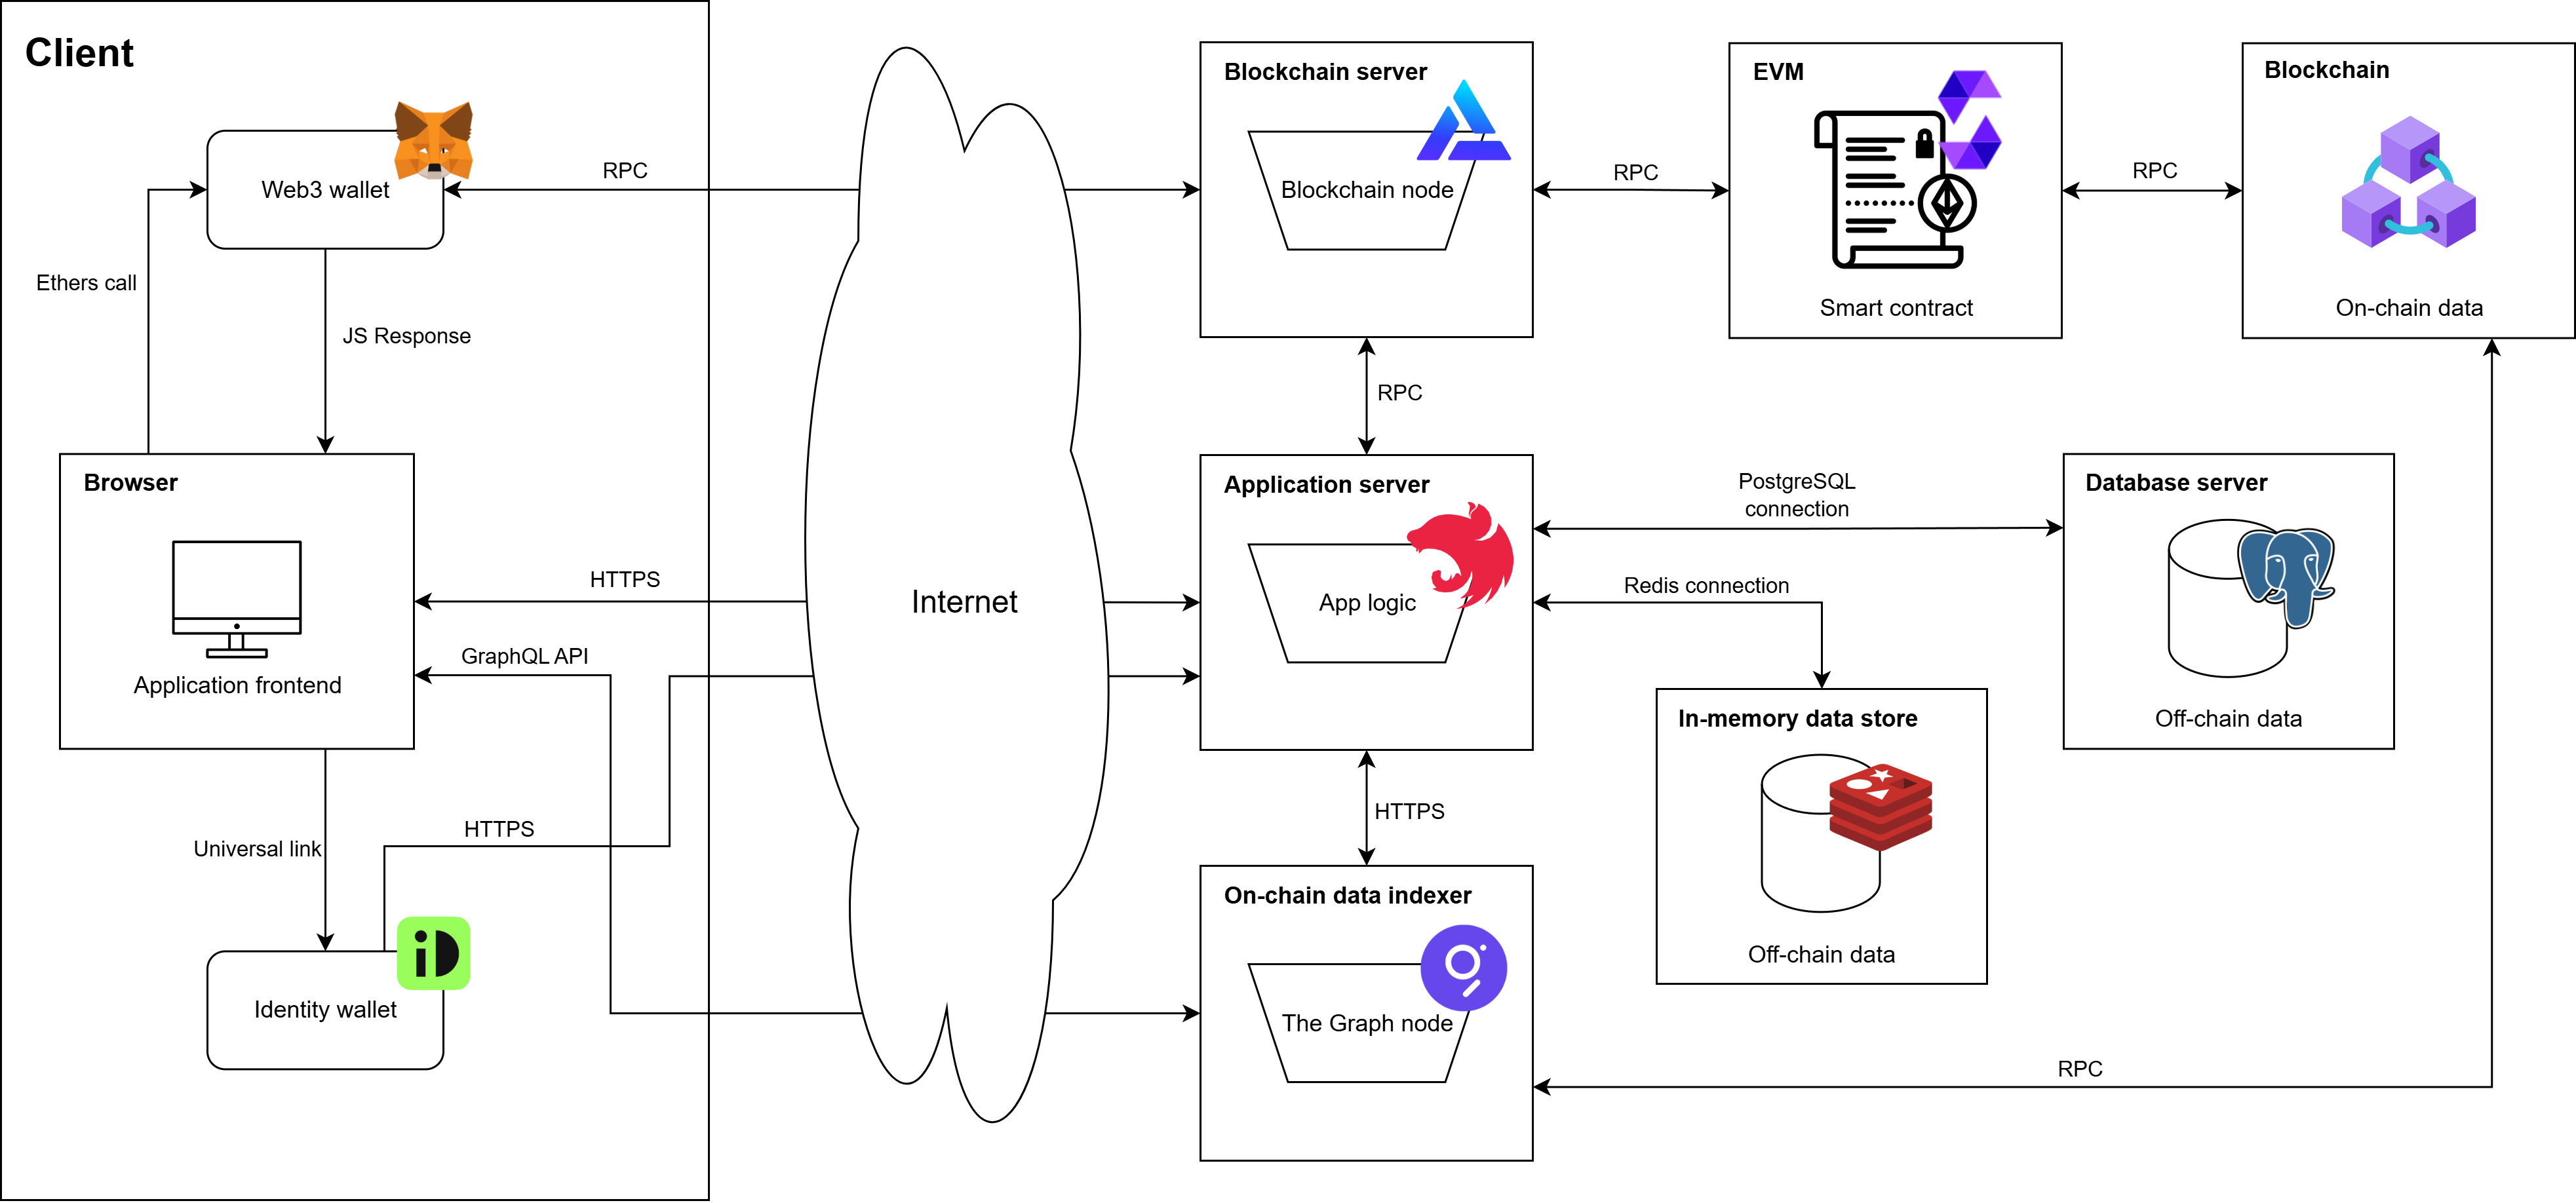
\includegraphics[width=0.99\linewidth]{architecture.png}
  \caption{System architecture diagram illustrating communication flow between key components. The front-end (Next.js) interacts with the back-end API (NestJS), which communicates with smart contracts deployed on the Ethereum Virtual Machine (EVM). SSI wallets and ZKP frameworks operate in parallel to provide verifiable credential handling and privacy-preserving interactions.}
  \label{fig:architecture_diagram}
\end{figure}

The architecture consists of the following layers:

\begin{enumerate}
  \item \textbf{Blockchain Layer:} An Ethereum-compatible blockchain handles deployment and execution of smart contracts for property listing, booking transactions, and dispute resolution. These contracts guarantee transparency, immutability, and censorship resistance \cite{buterin2014, wood2022, antonopoulos2019}.

  \item \textbf{SSI and ZKProof Layer:} Each user controls their identity via Decentralized Identifiers (DIDs) and Verifiable Credentials (VCs), issued according to W3C standards \cite{reed2020, sporny2022}. Credentials are stored in SSI-compatible wallets such as Privado ID \cite{iden3docs, mittal2025}, and proofs of claims are submitted using zk-SNARKs to maintain privacy \cite{chen2022, dieye2023, moya2023}.

  \item \textbf{Centralized System Layer:} Some functionalities—such as application logic, off-chain storage, and API services—are managed by centralized infrastructure hosted on cloud environments. This layer ensures scalability and performance while maintaining privacy through selective disclosure and ZKProof mechanisms.
\end{enumerate}

\subsection{User Roles and Responsibilities}

The system is built around the Self-Sovereign Identity (SSI) trust triangle and defines three primary user roles:

\begin{itemize}
  \item \textbf{Guests} are accommodation seekers who generate and manage verifiable credentials (VCs) on their devices. They prove claims such as booking validity or KYC status using zero-knowledge proofs (ZKPs) without exposing underlying data.
  \item \textbf{Hosts} offer property listings through the front-end interface and receive payments directly via smart contracts. They verify guest claims cryptographically, without requiring access to user identity data.
  \item \textbf{Platform operators} serve as credential issuers and oversee governance aspects such as dispute resolution. However, due to the system’s privacy-centric design, they cannot view or store personal data.
\end{itemize}

\subsection{Booking Credential Workflow}
Figure~\ref{fig:booking_communication_diagram} illustrates the credential issuance and verification flow during the booking process. In this model, the platform operator issues a booking credential to the guest upon successful reservation. The guest, as the holder, stores this credential in their digital wallet and presents a ZKP to the host to confirm the booking at check-in.

\begin{figure}[h!]
  \centering
  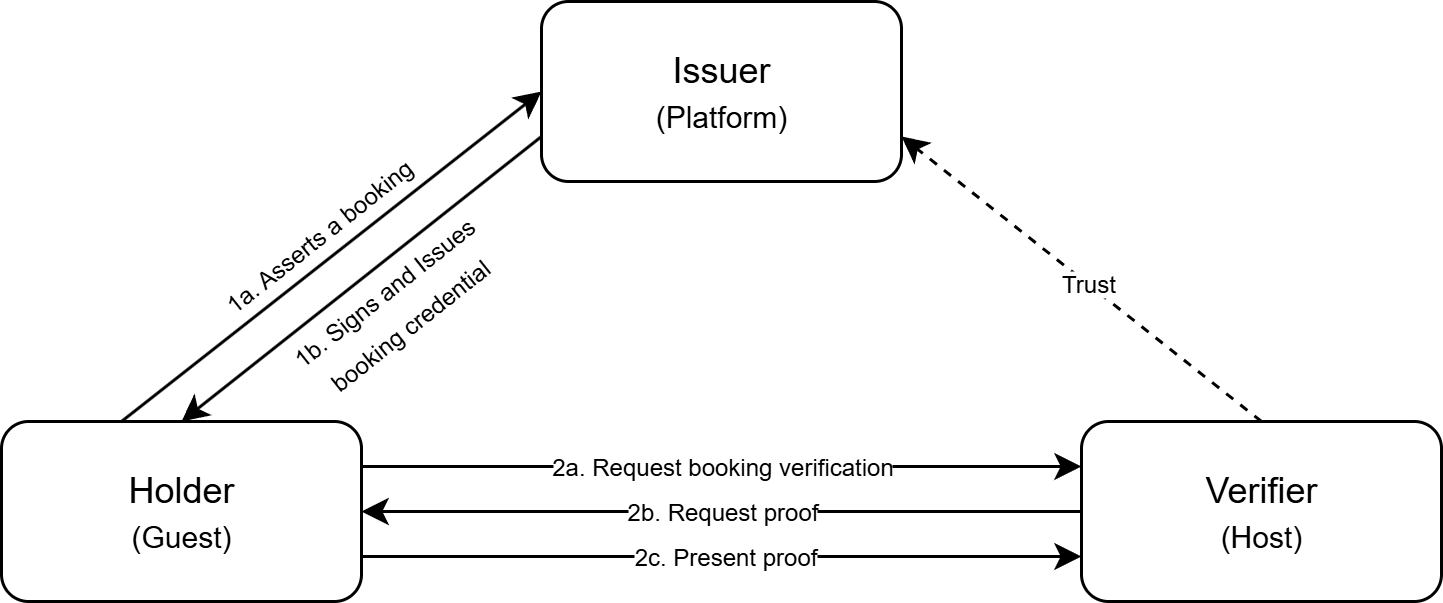
\includegraphics[width=0.99\linewidth]{communication-booking.png} % <- replace with correct image filename
  \caption{Booking credential issuance and verification flow based on the SSI trust triangle. Guests receive VCs from the platform and prove booking ownership to hosts via ZKP, with all verification performed on-chain.}
  \label{fig:booking_communication_diagram}
\end{figure}

This workflow ensures private, verifiable proof of reservation without revealing booking details or personal information. All verification logic is handled by smart contracts, ensuring trustless and tamper-proof validation.

\subsection{KYC Verification Workflow}
Figure~\ref{fig:kyc_communication_diagram} demonstrates how KYC verification is integrated into the platform using the same SSI structure. Instead of manually submitting identity documents to a centralized server, the guest completes KYC through an external trusted identity provider. The platform then issues a KYC-verification credential, which the user stores in their wallet.

\begin{figure}[h!]
  \centering
  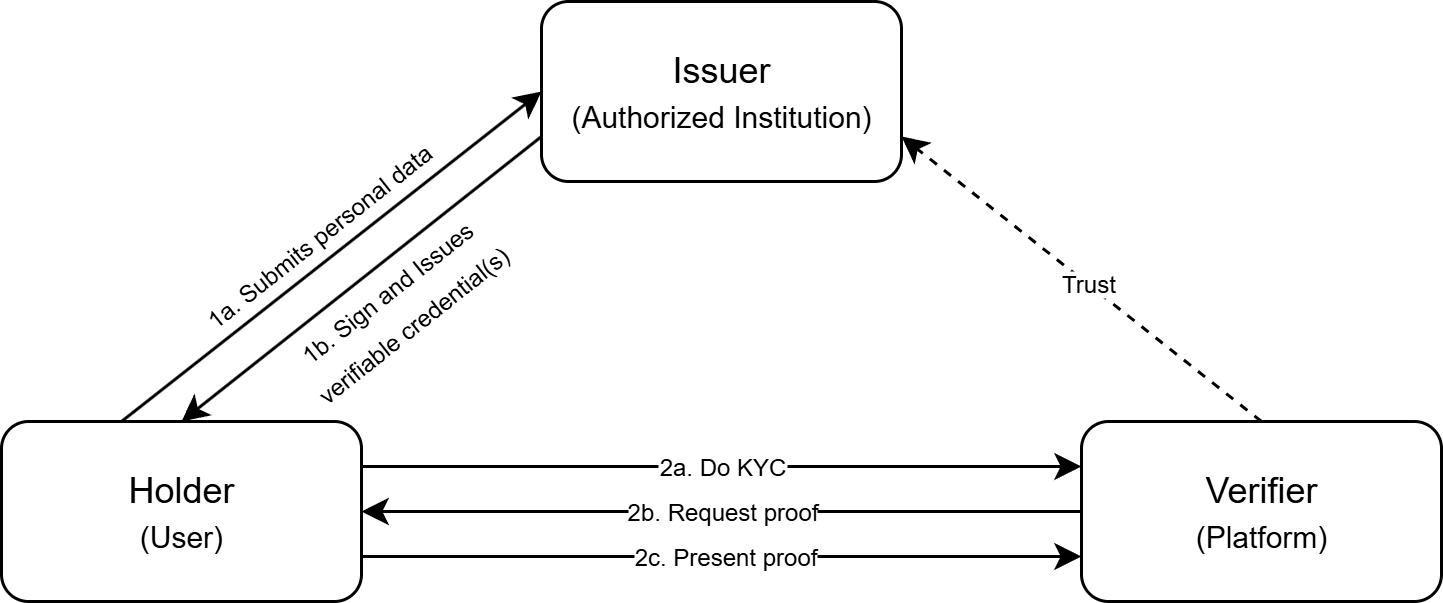
\includegraphics[width=0.99\linewidth]{communication-kyc.png} % <- replace with correct image filename
  \caption{KYC verification workflow. A trusted identity provider performs off-chain verification and the platform issues a credential. Guests can prove their KYC status to hosts without exposing sensitive data.}
  \label{fig:kyc_communication_diagram}
\end{figure}

This approach allows guests to cryptographically prove that they have completed KYC without disclosing personal identity attributes. Hosts gain confidence in user authenticity, while users retain control over their information.

\section{Implementation}
\label{sec:implementation}
\subsection{System Overview}
The P2P accommodation platform developed in this research introduces an \textit{innovation of meaning}, as described by Verganti~\cite{verganti2016}. Rather than offering merely a new technical solution, it redefines the meaning of trust in accommodation systems — from centralized identity control to user-sovereign, privacy-respecting interactions. Table~\ref{tab:comparison} compares conventional P2P AP platforms with the developed system.

\begin{table}[ht]
\caption{Comparison Between Traditional and Proposed P2P AP}
\label{tab:comparison}
\small
\begin{tabularx}{\columnwidth}{|p{2.5cm}|>{\raggedright\arraybackslash}X|>{\raggedright\arraybackslash}X|}
\hline
\textbf{Aspect} & \textbf{Traditional P2P AP} & \textbf{Proposed System} \\
\hline
Meaning of trust & Built through centralized authority and manual KYC & Built via cryptographic proofs (ZKProof) without centralized authority \\
\hline
Identity control & Managed and stored by the platform & Fully controlled by users via SSI \\
\hline
User privacy & Vulnerable to data misuse and leakage & Protected via selective disclosure and zero-knowledge proofs \\
\hline
Third-party role & Highly dependent on intermediaries & Minimized through autonomous, transparent smart contracts \\
\hline
Booking ownership & Stored in platform's internal database & Proven through on-chain verifiable credentials \\
\hline
User reputation & Moderated by centralized platform & Built on-chain based on transaction outcomes \\
\hline
Data ownership & Held by the platform & Owned by users (self-sovereign) \\
\hline
\end{tabularx}
\end{table}

This system eliminates the need to trust centralized entities by allowing users to prove important claims such as identity uniqueness, KYC status, and booking ownership through cryptographic means. It employs \textbf{Verifiable Credentials (VCs)} and \textbf{Zero-Knowledge Proofs (ZKPs)} to enable privacy-preserving authentication without disclosing sensitive data.

Smart contracts, deployed on the Ethereum blockchain, serve as the backbone of autonomous interactions. They facilitate transactions, record behavior for reputation, and resolve disputes — all without a centralized mediator. As a result, user reputations are transparently maintained on-chain, increasing accountability while ensuring decentralization.

This transition from "trust in authority" to "trust in protocol" embodies a paradigm shift, providing users with digital autonomy, stronger privacy, and decentralized control over their interactions within the accommodation ecosystem.

\subsection{Implementation Environment}
\label{subsec:environment}
The implementation environment includes the hardware and software components used during development, testing, and deployment. Table~\ref{tab:environment} summarizes the technical stack selected based on compatibility with blockchain, smart contract development, and web technologies.

\begin{table}[ht]
\caption{Implementation Environment}
\label{tab:environment}
\small
\begin{tabularx}{\columnwidth}{|p{3.5cm}|X|}
\hline
\textbf{Component Type} & \textbf{Tools / Technologies Used} \\
\hline
Development tools & Visual Studio Code, Subgraph Studio, TablePlus \\
\hline
Operating system & Windows \\
\hline
Database management system & PostgreSQL \\
\hline
Programming languages & TypeScript, Solidity \\
\hline
Query languages & GraphQL, SQL \\
\hline
Version control & GitHub \\
\hline
\end{tabularx}
\end{table}

\subsection{Deployment}
\label{subsec:deployment}
The system has been deployed and is publicly accessible. Smart contracts are deployed to the Ethereum Sepolia testnet. Frontend source code is available at \cite{ta-frontend}, while the backend logic and smart contracts are provided in \cite{ta-backend, ta-smartcontract}. Table~\ref{tab:deployment} provides the blockchain explorer links for the deployed smart contracts.

\begin{table}[ht]
\caption{Smart Contract Addresses}
\label{tab:deployment}
\small
\begin{tabularx}{\columnwidth}{|p{2.8cm}|X|}
\hline
\textbf{Smart Contract} & \textbf{Blockchain Explorer Link} \\
\hline
\texttt{RentalPayments} & \url{https://eth-sepolia.blockscout.com/address/0x0229E7dB6195A98D02aAe044C40D452e9f559A22} \\
\hline
\texttt{HostStake} & \url{https://eth-sepolia.blockscout.com/address/0xFf1a346fE650cef5100240A91c96A063CDe72C84} \\
\hline
\end{tabularx}
\end{table}

\section{Evaluation}
\label{sec:evaluation}

The P2P accommodation platform has successfully fulfilled its primary objectives, as confirmed by both functional testing and security analysis. Core processes—such as identity verification, booking, and payment—were executed autonomously via smart contracts without requiring third-party intervention. The system preserves user privacy by avoiding off-chain identity data storage.

Based on gas reports collected during unit testing, the average gas consumption for critical functions was significantly below the Ethereum block gas limit (30 million gas). Specifically:
\begin{itemize}
  \item \texttt{initiatePayment}: 197,881 gas
  \item \texttt{releasePayment}: 79,543 gas
  \item \texttt{resolveDispute}: 60,428 gas
\end{itemize}

These results indicate that all operations can be executed within a single block without risk of gas exhaustion. The \texttt{RentalPayments} contract utilizes only approximately 10.4\% of the block gas limit, while the \texttt{HostStake} contract consumes merely 3.8\%, confirming their efficiency, cost-effectiveness, and scalability.

Security evaluation was performed using \textbf{Slither}, a popular static analysis tool for Solidity smart contracts. The results showed no critical vulnerabilities such as reentrancy, integer overflows, or unauthorized state modifications. Minor issues and code smells were reviewed and either mitigated or determined to be non-impactful in the current deployment context.

Overall, the system demonstrates solid functional and security foundations, validating its feasibility as a proof-of-concept for a decentralized, privacy-preserving accommodation platform.

\section{Conclusion}
\label{sec:conclusion}
This research presents a decentralized peer-to-peer accommodation platform that redefines the notion of trust in digital interactions. Unlike traditional systems that depend on centralized authorities for identity verification, data storage, and reputation management, the proposed system leverages a combination of Self-Sovereign Identity (SSI), Zero-Knowledge Proofs (ZKP), and smart contracts to establish a trust-free environment that upholds user privacy, autonomy, and transparency.

The implementation demonstrates that it is feasible to design a platform where users can verify claims—such as KYC status and booking ownership—without revealing sensitive data. Verifiable Credentials (VCs) and ZKPs allow for selective disclosure and anonymous proof, while smart contracts automate transactions, reduce reliance on intermediaries, and provide a tamper-proof audit trail. By moving away from centralized control, the system introduces a new paradigm of trust, built on cryptographic assurances and user empowerment.

This innovation of meaning not only addresses long-standing concerns about privacy, security, and data ownership in platform economies but also introduces a scalable architectural model for future decentralized applications. The results suggest that blockchain-based trust frameworks, when combined with privacy-preserving identity protocols, can significantly enhance both user agency and system integrity in digital marketplaces.

Future work may involve evaluating user experience, stress-testing the protocol under large-scale adoption, and integrating additional verifiable attributes such as behavioral reputation or cross-platform credentials. Nonetheless, this research affirms the potential of decentralized identity and cryptographic proofs in reshaping how we trust and interact in online ecosystems.

\section*{Acknowledgment}
The author would like to express sincere gratitude to Ir. Budi Rahardjo, M.Sc., Ph.D., for his invaluable guidance and support throughout this thesis. Special thanks are also extended to Yudi Xu for his mentorship and practical insights, which greatly contributed to the implementation process.

Appreciation is due to the faculty and staff of the Information Systems and Technology program at Institut Teknologi Bandung for their knowledge and inspiration during the author's academic journey.

Heartfelt thanks go to the author’s family for their unwavering love and encouragement, and to close friends for their constant support and humor along the way.

\begin{thebibliography}{99}
\bibitem{rosoon2023} Y. Rosoon et al., "Decentralized Trusted Database," in \textit{Proc. ICITEE 2023}, pp. 282–286.
\bibitem{raj2019} K. Raj, \textit{Foundations of Blockchain}. Packt Publishing, 2019.
\bibitem{rundle2024} J. Rundle, "Finastra Hack," \textit{WSJ}, Nov. 2024.
\bibitem{malcolm2024} J. Malcolm, "Fidelity confirms 77,000 data breach," \textit{The Sun}, Oct. 2024.
\bibitem{blengini2024} I. Blengini and B. Venturini, "Transparency \& conflict resolution in Airbnb \& other two-sided markets," \textit{EHL Insights}, Mar. 2024.
\bibitem{hawlitschek2018} F. Hawlitschek et al., "The limits of trust-free systems," \textit{Electron. Commer. Res. Appl.}, vol. 29, pp. 50–63, May 2018.
\bibitem{mayer1995} R. C. Mayer et al., "An Integrative Model of Organizational Trust," \textit{Acad. Manage. Rev.}, vol. 20, 1995.
\bibitem{oliveira2017} T. Oliveira et al., "Consumer trust in e-commerce," \textit{Comput. Hum. Behav.}, vol. 71, pp. 153–164, Jun. 2017.
\bibitem{agag2019} G. Agag and R. Eid, "Examining the antecedents and consequences of trust in the context of peer-to-peer accommodation," \textit{Int. J. Hosp. Manag.}, vol. 81, pp. 180–192, Aug. 2019.
\bibitem{tussyadiah2018} I. P. Tussyadiah and S. Park, "Trust in host descriptions," \textit{Tour. Manag.}, vol. 67, pp. 261–272, Aug. 2018.
\bibitem{zloteanu2021} M. Zloteanu et al., "Trust \& Reputation in the Sharing Economy," \textit{Front. Psychol.}, vol. 12, 2021.
\bibitem{huang2021} Y.-K. Huang, "Attribution Bias on Online Reputation Systems," SSRN, Apr. 2021.
\bibitem{bhushan2021} B. Bhushan et al., "Untangling blockchain technology: A survey," \textit{Comput. Electr. Eng.}, vol. 90, Mar. 2021.
\bibitem{nakamoto2008} S. Nakamoto, "Bitcoin: A Peer-to-Peer Electronic Cash System," 2008.
\bibitem{wood2022} G. Wood, "Ethereum: A Secure Decentralised Ledger," Oct. 2022.
\bibitem{buterin2014} V. Buterin, "Ethereum: A Next-Generation Smart Contract and Decentralized Application Platform," 2014.
\bibitem{wang2019} F. Wang and P. De Filippi, "Self-Sovereign Identity in a Globalized World," \textit{Front. Blockchain}, vol. 2, 2019.
\bibitem{raipurkar2023} A. R. Raipurkar et al., "Digital Identity System Using Blockchain-based SSI \& ZKP," in \textit{Proc. OCIT 2023}, pp. 611–616.
\bibitem{mittal2025} P. Mittal, "Privado ID Documentation," Jan. 2025. [Online]. Available: https://docs.privado.id/
\bibitem{dieye2023} M. Dieye et al., "A Self-Sovereign Identity Based on Zero-Knowledge Proof and Blockchain," \textit{IEEE Access}, vol. 11, pp. 49445–49455, 2023.
\bibitem{chen2022} T. Chen et al., "A Review of zk-SNARKs," arXiv:2202.06877, Feb. 2022.
\bibitem{moya2023} C. V. Moya et al., "ZK Protocols on SSI Blockchain," \textit{Appl. Sci.}, vol. 13, no. 9, 2023.
\bibitem{lux2020} A. Z. Lux et al., "DL-based Authentication with DIDs and VCs," \textit{IEEE}, 2020.
\bibitem{sporny2022} M. Sporny, D. Longley, and D. Chadwick, "Verifiable Credentials Data Model v1.1," W3C, Mar. 2022.
\bibitem{reed2020} D. Reed et al., "Decentralized Identifiers (DIDs) v1.0," W3C, Oct. 2020.
\bibitem{peffers2007} K. Peffers et al., "A Design Science Research Methodology," \textit{J. Manag. Inf. Syst.}, vol. 24, no. 3, pp. 45–77, 2007.
\bibitem{venable2017} J. R. Venable et al., "Choosing a DSR Methodology," in \textit{ACIS 2017}.
\bibitem{cesnuityte2022} V. Česnuitytė et al., \textit{The Sharing Economy in Europe}. Springer, 2022.
\bibitem{antonopoulos2019} A. M. Antonopoulos and G. D. Wood, \textit{Mastering Ethereum}. The Ethereum Book LLC, 2019.
\bibitem{solidity2024} Solidity, "Solidity Documentation Release 0.8.29," 2024. [Online]. Available: https://docs.soliditylang.org/
\bibitem{xu2014} J. Xu et al., "How users develop trust in technology," \textit{Appl. Ergon.}, vol. 45, no. 6, pp. 1495–1503, 2014.
\bibitem{gan2024} Q. Q. Gan and R. Y. K. Lau, "Trust in a 'trust-free' system: Blockchain acceptance," \textit{Tech. Forecast. Soc. Change}, vol. 199, Feb. 2024.
\bibitem{iden3docs} Iden3, "Iden3 Documentation," 2023. [Online]. Available: https://docs.iden3.io/
\bibitem{cheqd2023} cheqd, ``Self-sovereign identity explained,'' cheqd.io, 2023. [Online]. Available: \url{https://cheqd.io/ssi/}. [Accessed: 18-Jul-2025].
\bibitem{dann2020} D. Dann et al., "Blockchain and Trust in the Platform Economy," in \textit{WI2020}, pp. 1459–1473, 2020.
\bibitem{verganti2016} R. Verganti, \textit{Overcrowded: Designing Meaningful Products in a World Awash with Ideas}. Cambridge, MA: MIT Press, 2016.
\bibitem{ta-frontend} Ceavin Rufus, "TA Frontend Repository: User Interface for P2P Accommodation Platform," GitHub, 2025. [Online]. Available: \url{https://github.com/ceavinrufus/TA-frontend} [Accessed: 18-Jul-2025].
\bibitem{ta-backend} Ceavin Rufus, "TA Backend Repository: API and Server Logic for P2P Accommodation Platform," GitHub, 2025. [Online]. Available: \url{https://github.com/ceavinrufus/TA-backend} [Accessed: 18-Jul-2025].
\bibitem{ta-smartcontract} Ceavin Rufus, "TA Smart Contract Repository: Ethereum Contracts for P2P Accommodation Platform," GitHub, 2025. [Online]. Available: \url{https://github.com/ceavinrufus/TA-smart-contract} [Accessed: 18-Jul-2025].
\end{thebibliography}

\end{document}
